\section{Polygonal Linkages}

\begin{figure}[h]
\begin{center}

\includegraphics[scale=1]{graphics/hingeOnThreeDistinctPolygons.pdf}
\end{center} 
\caption{(a) A polygonal linkage with a non-convex polygon and two hinge points corresponding to 
three polygons.  Note that hinge points correspond to two distinct polygons.(b) Illustrating that 
two hinge points can correspond to the same boundary point of a polygon.}
\label{fig:linkage-1}
\end{figure}
%describe how it is a generalization of Linkages.
A generalization of linkages are polygonal linkages where the edges of given lengths are replaced 
by rigid polygons.  Formally, a \textit{polygonal linkage} is an ordered pair $\left(\PP,\HH 
\right)$ where $\PP$ is a finite set of polygons and $\HH$ is a finite set of hinges; a 
\textit{hinge} $h\in \HH$ 
corresponds to two points on the boundary of two distinct polygons in $\PP$.  A \emph{realization} 
of a polygonal linkage is an interior-disjoint placement of 
congruent copies of the polygons in $\PP$ such that the points corresponding to each hinge are 
identified (Fig. \ref{fig:1}). 
A \textbf{realization with orientation} uses only translated or rotated copies of the polygons in $\PP$ (no reflections) and for each hinge, the cyclic order of incident polygons is given. 
The topology of a polygonal linkage can be represented by the \textbf{hinge graph}, a bipartite graph where the vertices correspond to polygons in $\PP$ and the hinges in $H$, and edges represent the polygon-hinge incidences.
This definition of realization rules well known geometric 
dissections (e.g. Fig. \ref{fig:polygonallinkage-4}).
%this is where the geometric dissection figure belongs
\begin{figure}[h]
\begin{center}
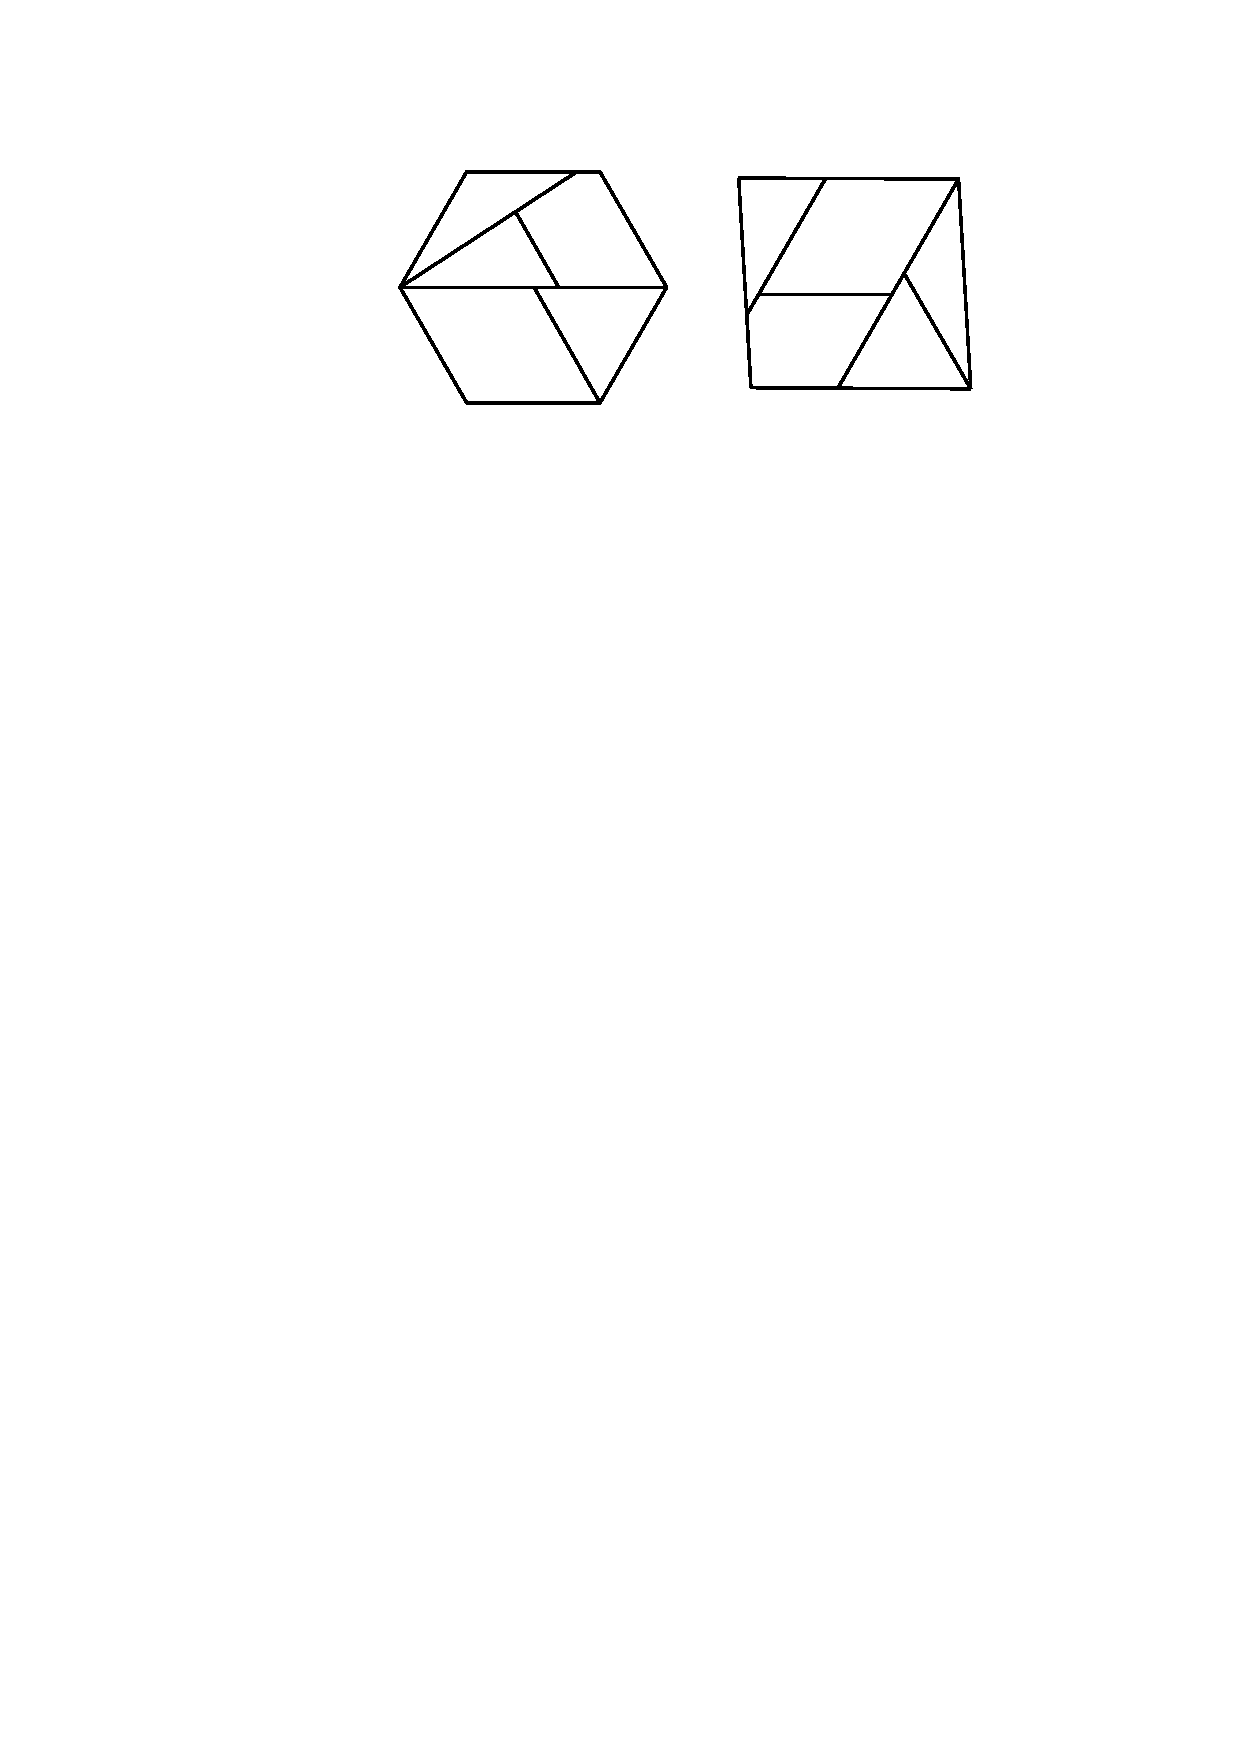
\includegraphics{graphics/GeometricDissectionBusschop.pdf}
\end{center}
\caption{Two configurations of polygonal linkage where the polygons touch on boundary segments 
instead of hinges.  These two realizations of the polygonal linkage are invalid to our definitions. 
 }
\label{fig:polygonallinkage-4}
\end{figure}

\begin{figure}[h]
\begin{center}
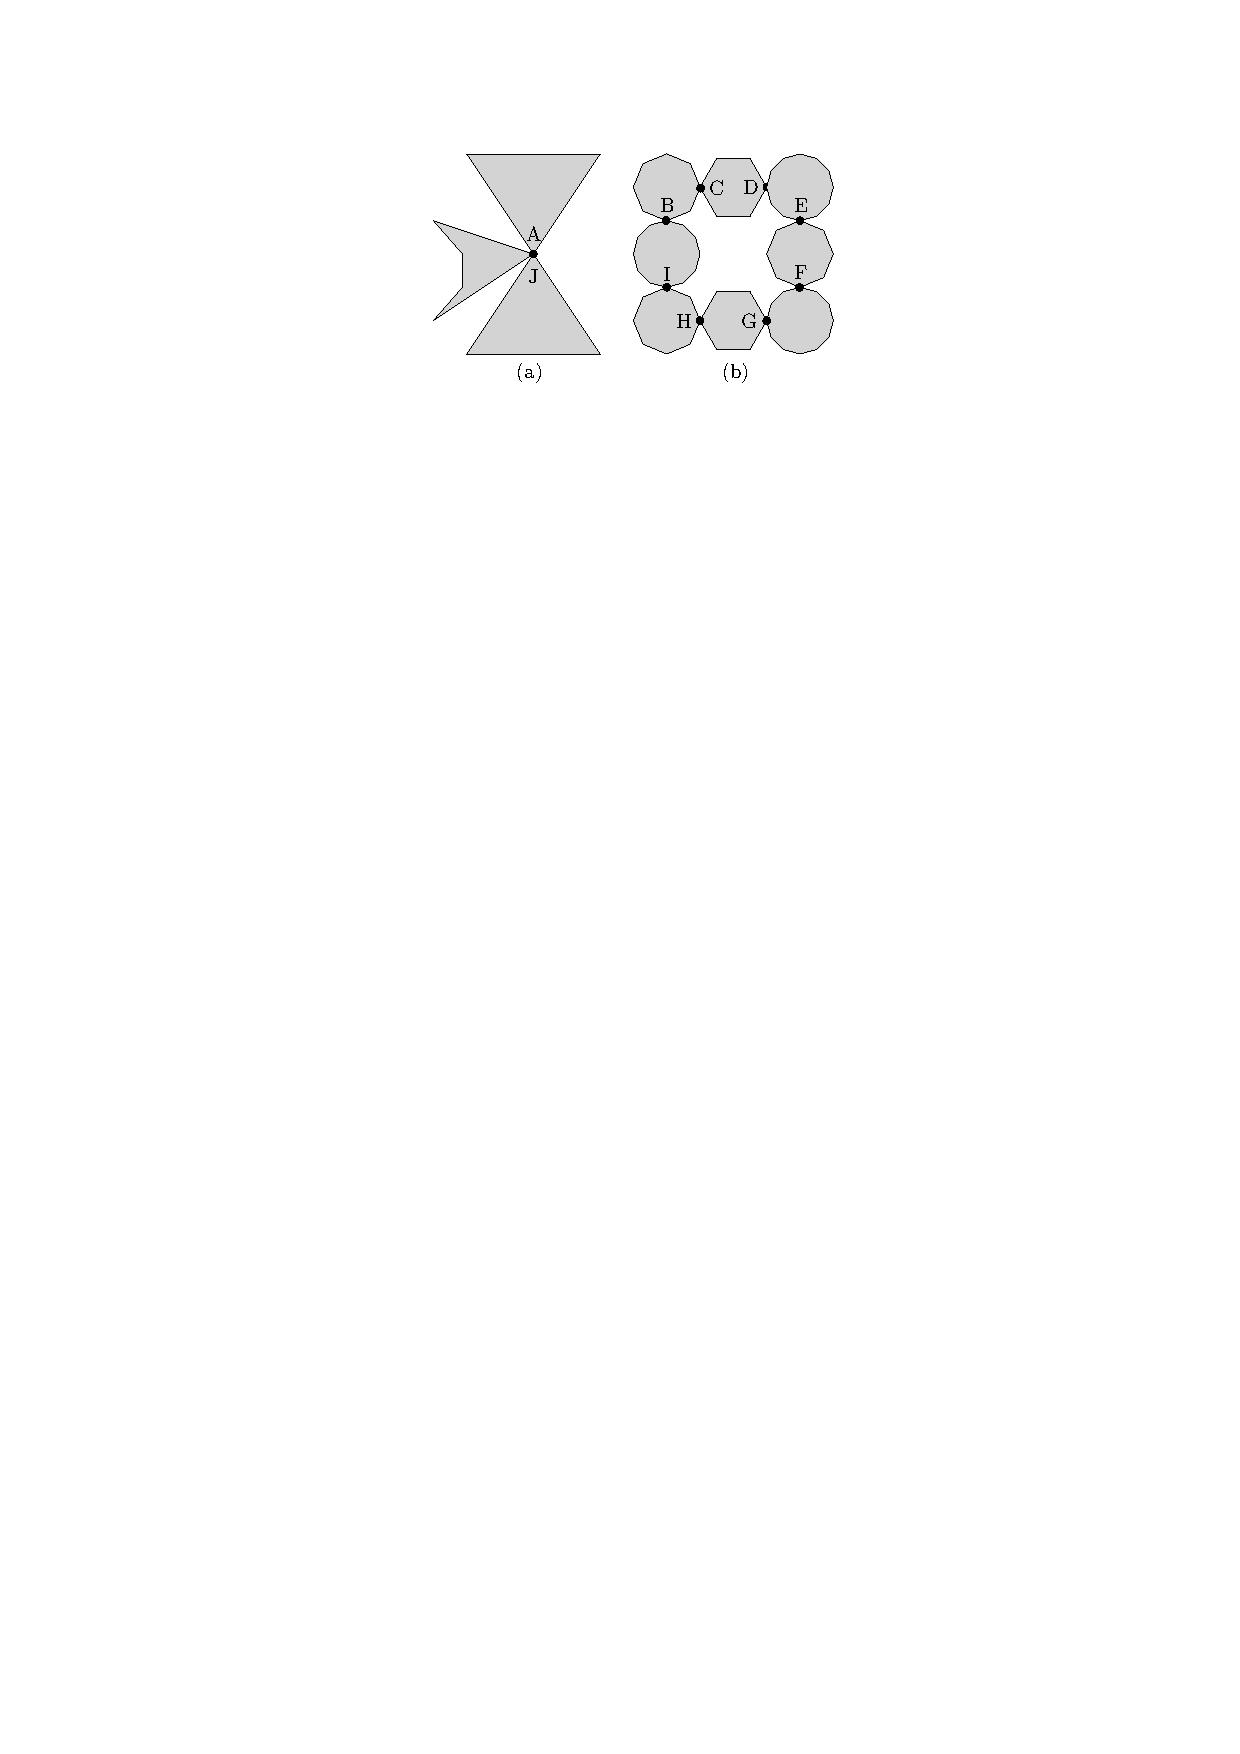
\includegraphics[scale=1]{graphics/linkageillustration.pdf}
\end{center} 
\caption{(a) A polygonal linkage with a non-convex polygon and a hinge point corresponding to three 
polygons.  (b) A polygonal linkage with 8 regular polygons.}
\label{fig:linkage-2}
\end{figure}


% For the remainder of this thesis, we'll focus on the polygonal linkages with the following 
% restrictions:
% \begin{enumerate}
% \item Embedded polygons must be convex, i.e. for any two embedded points $u,v \in P'$, the set:
% $$\left\lbrace u  \cdot t + (1-t) \cdot v : t \in [0,1] \right\rbrace \in P'$$
%  \item  Polygons can only intersect at hinge points.  No two polygons can intersect at 
% their boundary or interior with the exception of possible a hinge point.  
% \end{enumerate}